%%%%%%%%%%%%%%%%%%%%%%%%%%%%%%%%%%%%%%%%%%%%%%%%%%%%%%%%%%%%%%%%%%%%%%
%%                           APPENDIX D
%%%%%%%%%%%%%%%%%%%%%%%%%%%%%%%%%%%%%%%%%%%%%%%%%%%%%%%%%%%%%%%%%%%%%

\chapter{\uppercase {Supplemental Data - Chapter Five}}

%%%%%%%%%%%%%%%%%%%%%%%%%%%%%%%%%%%%%%%%%%%%%%%%%%%%%%
\vspace*{\fill}
\begin{figure}[ht]
  \centering
  \resizebox{\linewidth}{!}{
    \begin{tikzpicture}[every label/.style={font=\Large\bfseries},node distance=2cm,text depth=0.25ex,pic/.style={inner sep=0pt}]
      \node[pic] (embryos)    [label={[label distance=1.1cm,text width=5cm]below:\emph{Ube3a$^{YFP}$} Embryos Collected}] {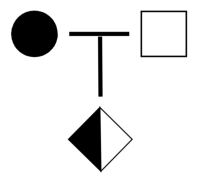
\includegraphics[width=0.25\textwidth]{figures/embryos-collected.pdf}};
      \node[pic] (blastocyst) [right= of embryos,label={[label distance=1cm,text width=4cm]below:Blastocyst Cultured}]    {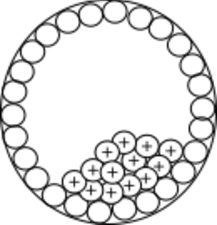
\includegraphics[width=0.25\textwidth]{figures/blastocyst.pdf}};
      \node[pic] (icm)        [right= of blastocyst,label={[label distance=2.3cm,text width=3cm]below:Isolation of ICM}]  {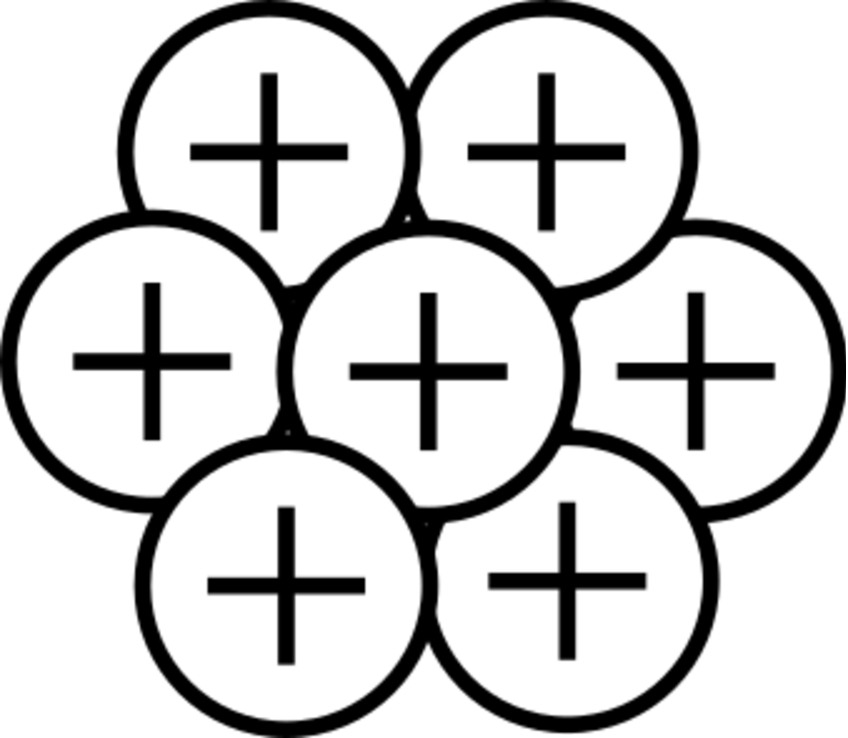
\includegraphics[width=0.10\textwidth]{figures/icm.pdf}};
      \node[pic] (cell)       [right= of icm,label={[label distance=2.35cm,text width=5cm]below:Cell Dissociated}]        {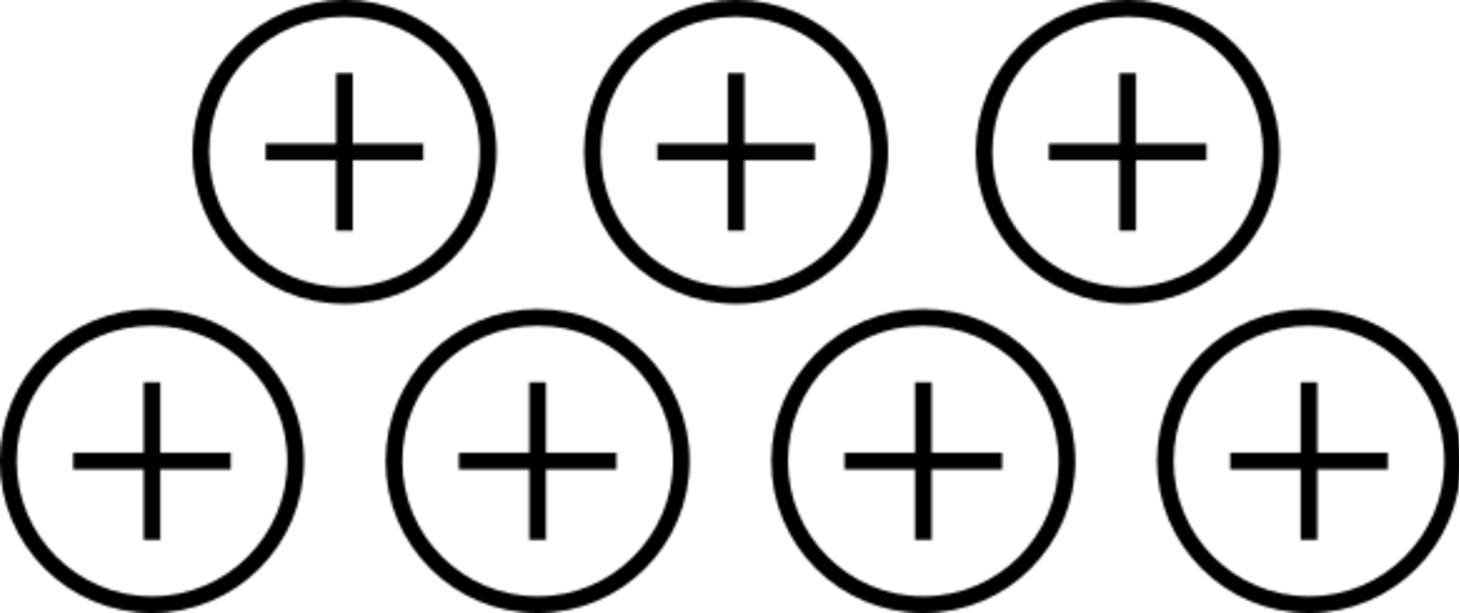
\includegraphics[width=0.20\textwidth]{figures/cell-dissociated.pdf}};
      \node[pic] (expansion)  [right= of cell,label={[label distance=1.05cm]below:Expansion}]                             {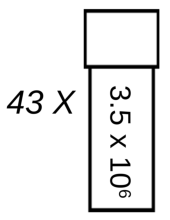
\includegraphics[width=0.20\textwidth]{figures/expansion.pdf}};

      \draw[line width=4pt,->] (embryos)    -- (blastocyst);
      \draw[line width=4pt,->] (blastocyst) -- (icm);
      \draw[line width=4pt,->] (icm)        -- (cell);
      \draw[line width=4pt,->] (cell)       -- (expansion);
      
    \end{tikzpicture}
  }
  \vspace*{5mm}
  \caption{Example schematic of \textit{Ube3a$^{YFP}$} embryonic stem cell generation and expansion.}
\end{figure}
%%%%%%%%%%%%%%%%%%%%%%%%%%%%%%%%%%%%%%%%%%%%%%%%%%%%%%

%%%%%%%%%%%%%%%%%%%%%%%%%%%%%%%%%%%%%%%%%%%%%%%%%%%%%%
\begin{figure}[ht]
  \centering
  \resizebox{6in}{!}{
    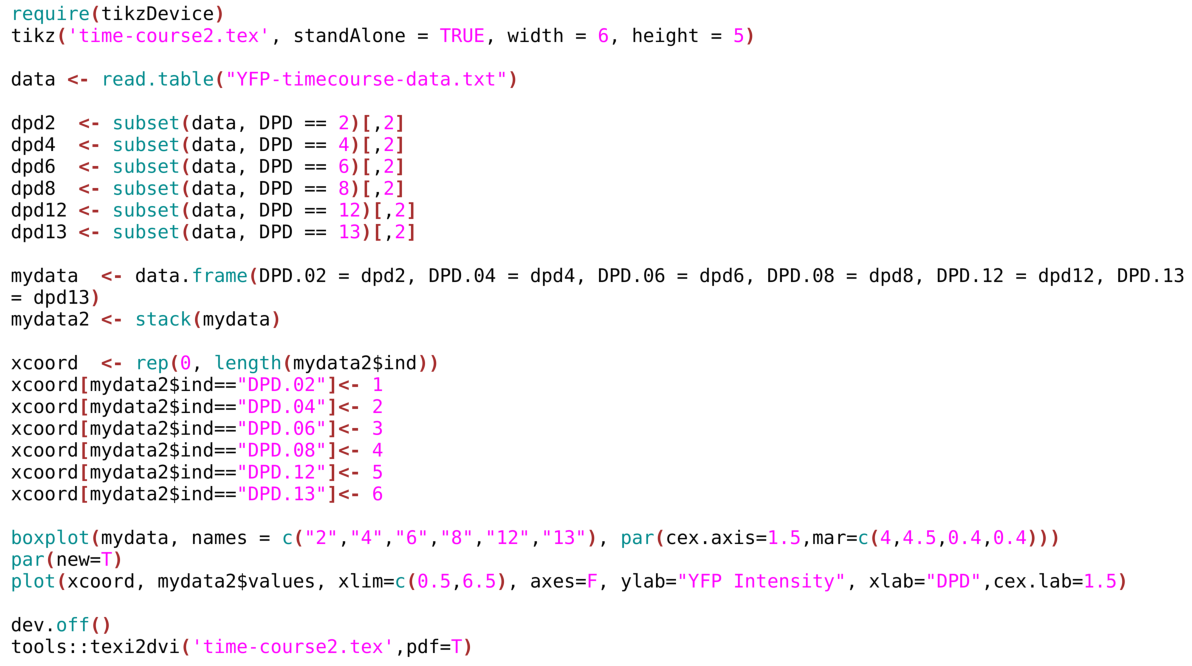
\includegraphics{figures/timecourse-R_edit.pdf}
  }
  \caption{Sample script for generating boxplots for embryonic stem cell-derived neurons time course}
\end{figure}
%%%%%%%%%%%%%%%%%%%%%%%%%%%%%%%%%%%%%%%%%%%%%%%%%%%%%%

%%%%%%%%%%%%%%%%%%%%%%%%%%%%%%%%%%%%%%%%%%%%%%%%%%%%%%
\begin{figure}[ht]
  \centering
    \begin{tikzpicture}[every label/.style={font=\Large\bfseries},text depth=0.25ex,pic/.style={inner sep=0pt}]
      \node[pic] (dpd2)  [label={[label distance=1mm]145:A}] {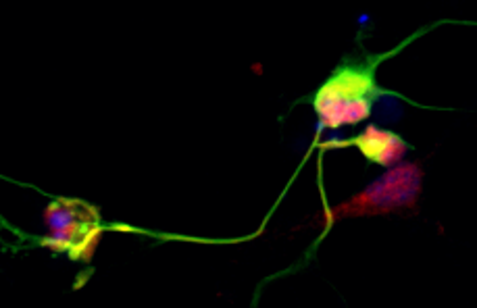
\includegraphics[width=0.40\textwidth]{figures/dpd2.pdf}};
      \node[pic] (dpd13) [below= 1mm of dpd2]                       {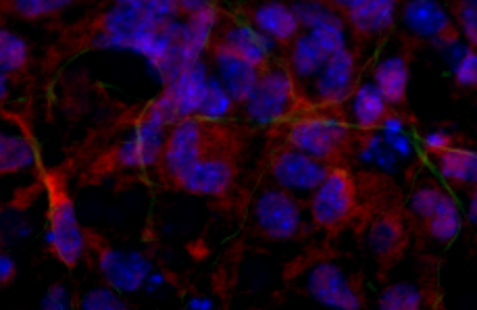
\includegraphics[width=0.40\textwidth]{figures/dpd13.pdf}};

      \begin{scope}[xshift=7cm]
        \node[pic] (off) [label={[label distance=1mm]145:B}] {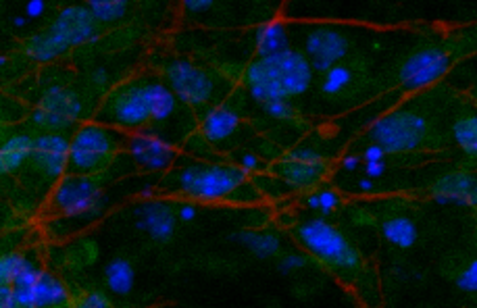
\includegraphics[width=0.40\textwidth]{figures/neuron-off.pdf}};
        \node[pic] (on)  [below= 1mm of off]                        {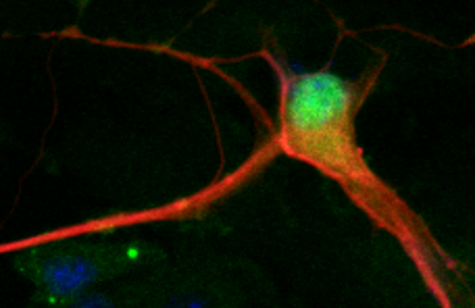
\includegraphics[width=0.40\textwidth]{figures/neuron-on.pdf}};
      \end{scope}
      
    \end{tikzpicture}
  \caption{Topotecan induces reactivation of paternal \emph{Ube3a} allele in ES cell-derived neurons. \textbf{A)} Confocal image (40X magnification) of \emph{Ube3a$^{YFP}$} ES cell-derived neurons at 2 and 13 days post dissociation (DPD) demonstrating the imprinting of paternal \emph{Ube3a}. Nuclei marker TO-PRO-3 (blue), GFP (red), and \( \beta \)III Tub (green). \textbf{B)} Confocal image (40X magnification) of ES cell-derived neurons at 13 DPD with vehicle (water) or Topotecan (300 nM) treatment demonstrating the reactivation of paternal \emph{Ube3a}. Nuclei marker TO-PRO-3 (blue), GFP (green), and \( \beta \)III Tub (red).}
\end{figure}
%%%%%%%%%%%%%%%%%%%%%%%%%%%%%%%%%%%%%%%%%%%%%%%%%%%%%%

%%%%%%%%%%%%%%%%%%%%%%%%%%%%%%%%%%%%%%%%%%%%%%%%%%%%%%
\begin{figure}[ht]
  \centering
  \resizebox{6in}{7in}{
    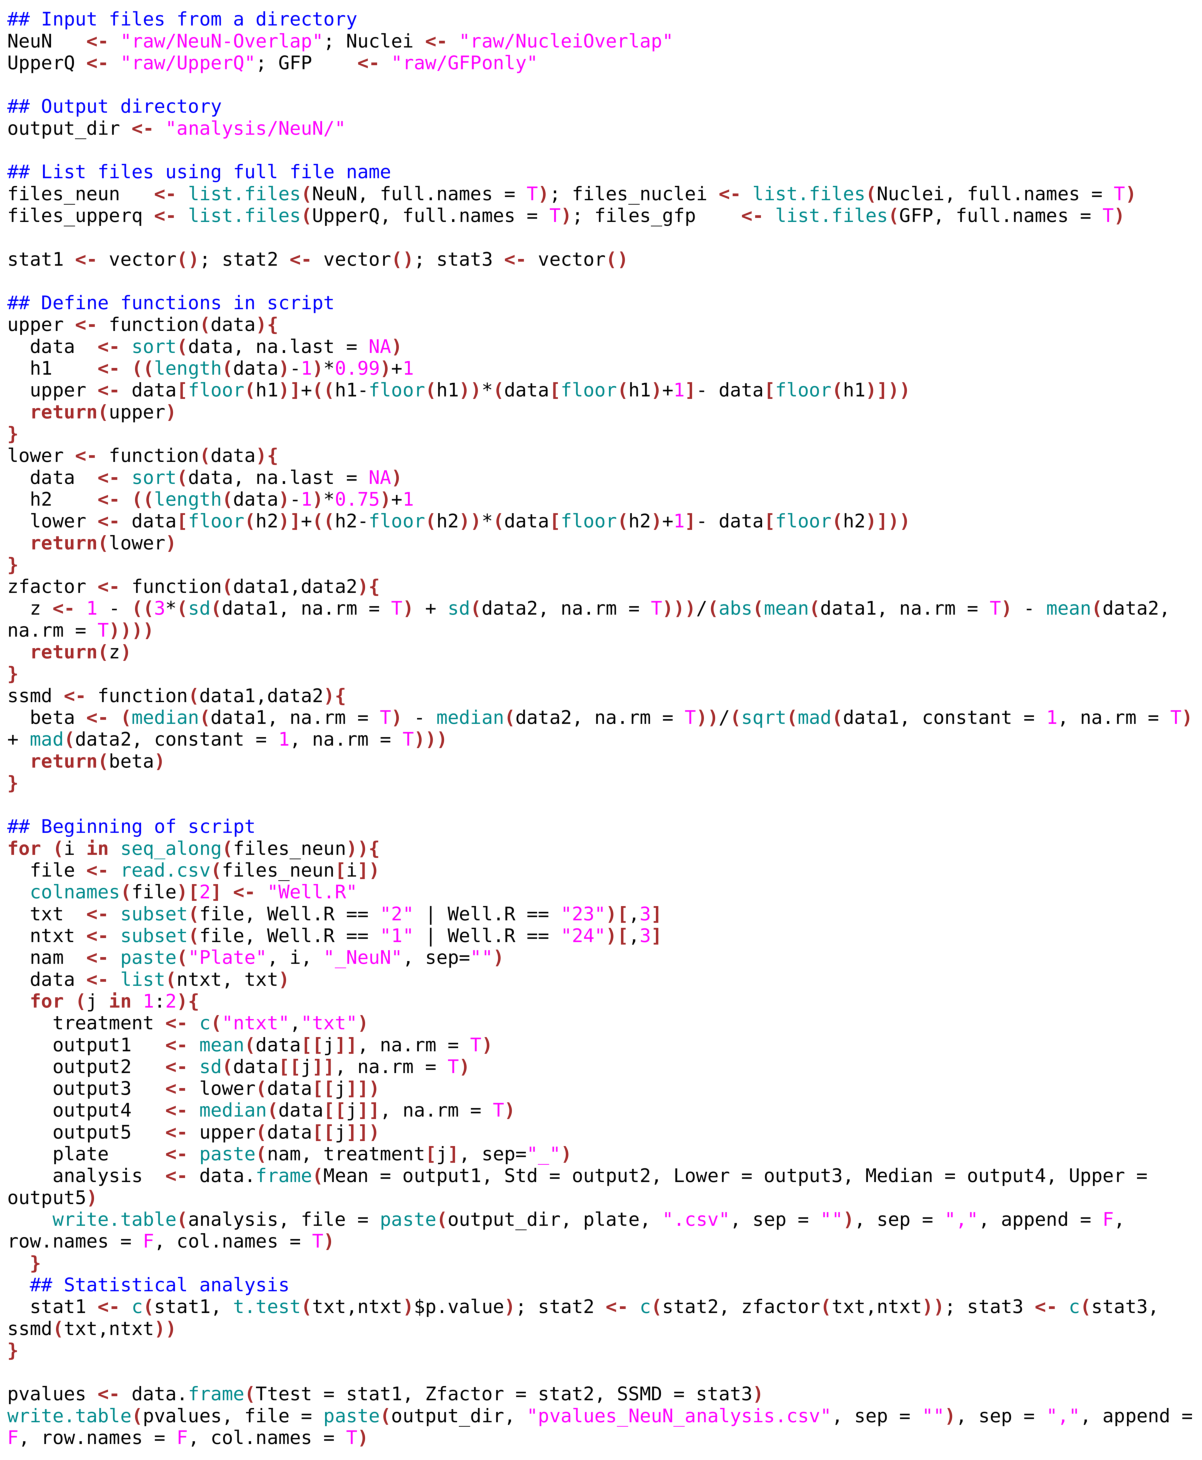
\includegraphics{figures/plate-analysis-R_edit.pdf}
  }
  \caption{Sample script for plate analysis}
\end{figure}
%%%%%%%%%%%%%%%%%%%%%%%%%%%%%%%%%%%%%%%%%%%%%%%%%%%%%%

%%%%%%%%%%%%%%%%%%%%%%%%%%%%%%%%%%%%%%%%%%%%%%%%%%%%%%
\begin{figure}[ht]
  \centering
  \resizebox{6in}{8in}{
    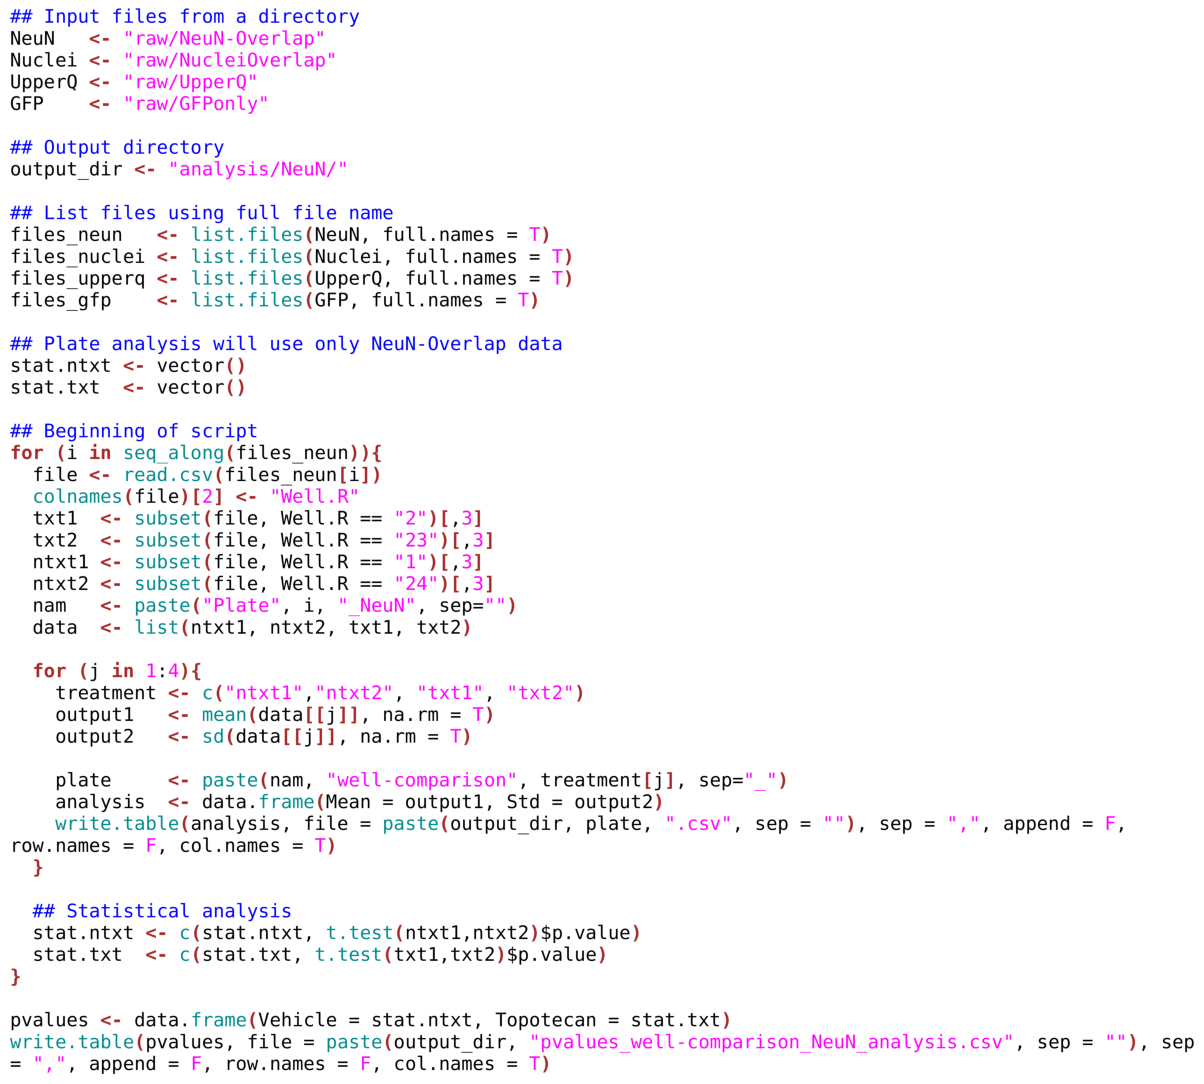
\includegraphics{figures/well-analysis-R_edit.pdf}
  }
  \caption{Sample script for well-effect analysis}
\end{figure}
%%%%%%%%%%%%%%%%%%%%%%%%%%%%%%%%%%%%%%%%%%%%%%%%%%%%%%

%%%%%%%%%%%%%%%%%%%%%%%%%%%%%%%%%%%%%%%%%%%%%%%%%%%%%%
\begin{sidewaysfigure}[ht]
  \centering
  \resizebox{\linewidth}{!}{
    \begin{tikzpicture}[every label/.style={font=\Large\bfseries},box/.style={text height=1.5ex, text depth=0.25ex}]
      \node[box]           (gfp)                        {\uline{\textbf{GFP Only}}};
      \node[box,rectangle] (process) [below=1mm of gfp] {Image Processing};
      \node[box,rectangle] (segment) [below=of process] {Target Segmentation};
      \node[box,rectangle] (data)    [below=of segment] {Collect Data};

      \draw[vecArrow]   (process) to (segment);
      \draw[vecArrow]   (segment) to (data);
      %% \draw[innerWhite] (process) to (segment);
      %% \draw[innerWhite] (segment) to (data);

      \begin{scope}[xshift=4.5cm]
        \node[box]           (nuclei)                         {\uline{\textbf{Nuclei-Overlap}}};
        \node[box,rectangle] (mask1)    [below=1mm of nuclei] {Nuclei Mask};
        \node[box,rectangle] (process1) [below=of mask1]      {Image Processing};
        \node[box,rectangle] (segment1) [below=of process1]   {Target Segmentation};
        \node[box,rectangle] (data1)    [below=of segment1]   {Collect Data};

        \draw[vecArrow] (mask1)    to (process1);
        \draw[vecArrow] (process1) to (segment1);
        \draw[vecArrow] (segment1) to (data1);
      \end{scope}
      \begin{scope}[xshift=9cm,yshift=-1.1cm]
        \node[box,rectangle]     (mask2)                                    {NeuN Mask};
        \node[box,rectangle]     (mask3)    [right=1cm of mask2]            {Nuclei Mask};
        \node[box,inner sep=0pt] (empty)    [above right=0.5mm of mask2]    {};
        \node[box]               (neun)     [above=0.5mm of empty]          {\uline{\textbf{NeuN-Overlap}}};
        \node[box,rectangle]     (process2) [below=of mask2]                {Image Processing};
        \node[box,rectangle]     (process3) [below=of mask3]                {Image Processing};
        \node[box,inner sep=0pt] (empty2)   [below right=6.0mm of process2] {};
        \node[box,rectangle]     (overlap)  [below=0.1mm of empty2]         {Overlapping Mask};
        \node[box,rectangle]     (segment2) [below=of overlap]              {Target Segmentation};
        \node[box,rectangle]     (data2)    [below=of segment2]             {Collect Data};

        \draw[vecArrow] (mask2)    to (process2);
        \draw[vecArrow] (mask3)    to (process3);
        \draw[vecArrow] (process2) to (overlap);
        \draw[vecArrow] (process3) to (overlap);
        \draw[vecArrow] (overlap)  to (segment2);
        \draw[vecArrow] (segment2) to (data2);
      \end{scope}
    \end{tikzpicture}
  }
  \vspace*{1mm}
  \caption{Flow chart of analysis methods. Note that UpperQ method uses the GFP only data set and collects data from the 75th to 99th percentile.}
\end{sidewaysfigure}
%%%%%%%%%%%%%%%%%%%%%%%%%%%%%%%%%%%%%%%%%%%%%%%%%%%%%%
\vspace*{\fill}
\begin{figure}[!ht]
  \centering
  \resizebox{\linewidth}{6in}{
    \begin{tikzpicture}[every label/.style={font=\Large\bfseries},pic/.style={inner sep=0pt}]
      \node[pic] [label={[label distance=2mm]above:Nuclei-Overlap}] {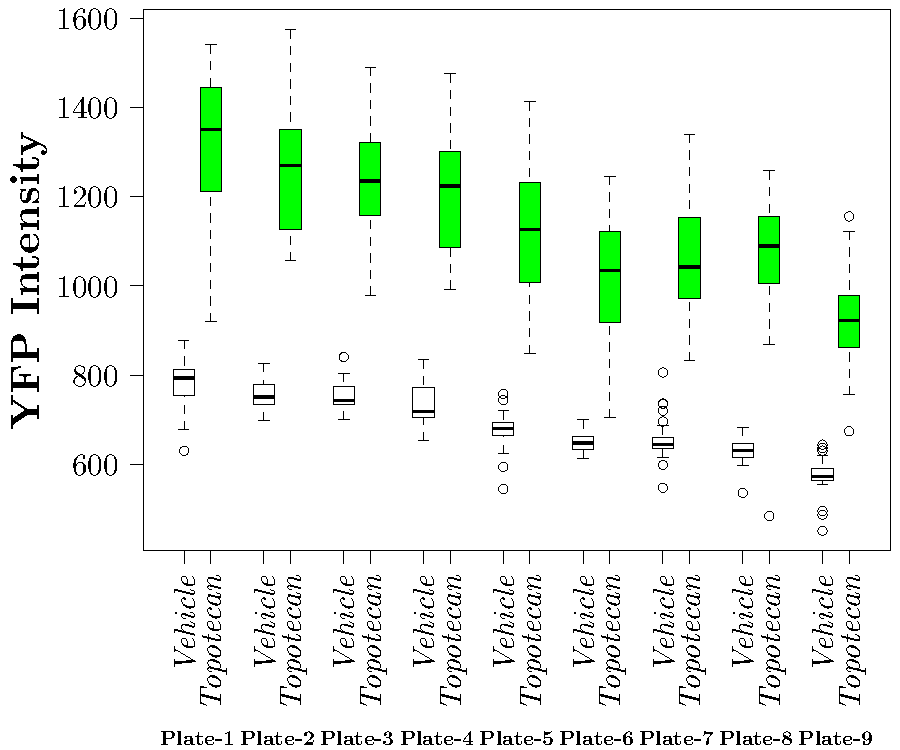
\includegraphics[width=0.90\textwidth]{figures/plate-analysis2.pdf}};
    \end{tikzpicture}
  }
  \vspace*{1mm}
  \caption{The decrease in Ube3a$^{YFP}$ intensity as a function of time, \textbf{Nuclei-Overlap} method.}
\end{figure}
\vspace*{\fill}
%%%%%%%%%%%%%%%%%%%%%%%%%%%%%%%%%%%%%%%%%%%%%%%%%%%%%%
\pagebreak
%%%%%%%%%%%%%%%%%%%%%%%%%%%%%%%%%%%%%%%%%%%%%%%%%%%%%%
\vspace*{\fill}
\begin{figure}[!ht]
  \centering
  \resizebox{\linewidth}{6in}{
    \begin{tikzpicture}[every label/.style={font=\Large\bfseries},pic/.style={inner sep=0pt}]
      \node[pic] [label={[label distance=2mm]above:UpperQ}] {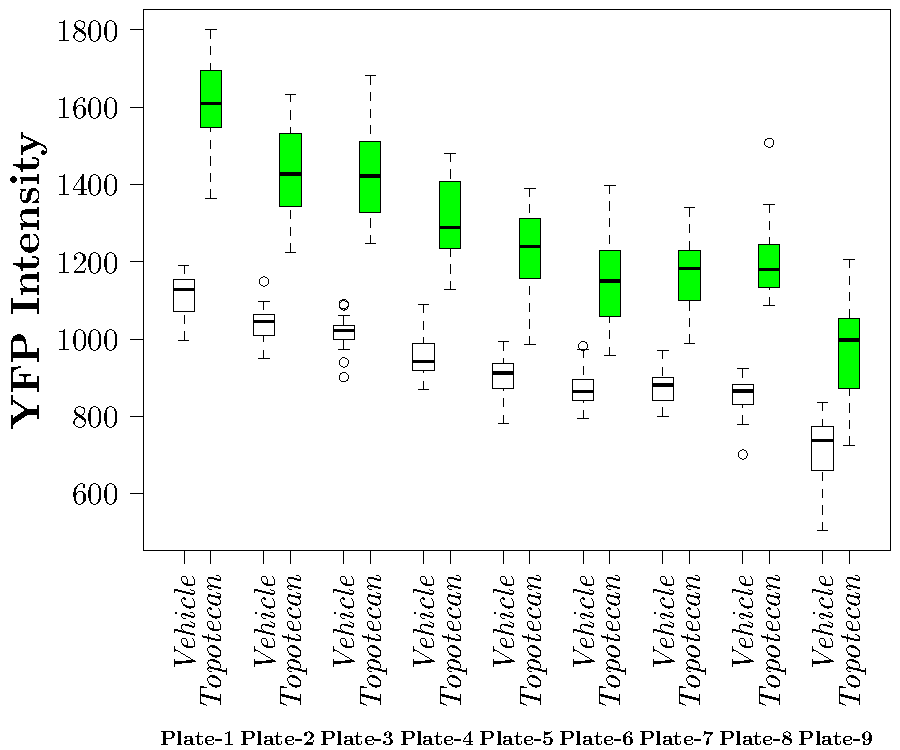
\includegraphics[width=0.90\textwidth]{figures/plate-analysis3.pdf}};
    \end{tikzpicture}
  }
  \vspace*{1mm}
  \caption{The decrease in Ube3a$^{YFP}$ intensity as a function of time, \textbf{UpperQ} method.}
\end{figure}
\vspace*{\fill}
%%%%%%%%%%%%%%%%%%%%%%%%%%%%%%%%%%%%%%%%%%%%%%%%%%%%%%
\pagebreak
%%%%%%%%%%%%%%%%%%%%%%%%%%%%%%%%%%%%%%%%%%%%%%%%%%%%%%
\vspace*{\fill}
\begin{figure}[!ht]
  \centering
  \resizebox{\linewidth}{6in}{
    \begin{tikzpicture}[every label/.style={font=\Large\bfseries},pic/.style={inner sep=0pt}]
      \node[pic] [label={[label distance=2mm]above:GFP only}] {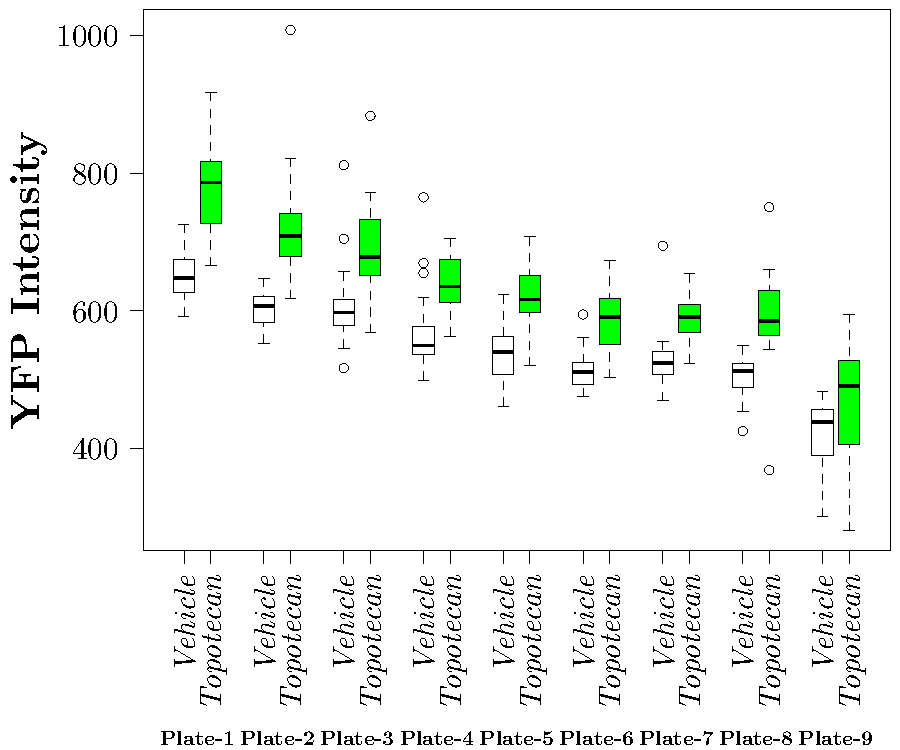
\includegraphics[width=0.90\textwidth]{figures/plate-analysis4.pdf}};
    \end{tikzpicture}
  }
  \vspace*{1mm}
  \caption{The decrease in Ube3a$^{YFP}$ intensity as a function of time, \textbf{GFP only} method.}
\end{figure}
\vspace*{\fill}
%%%%%%%%%%%%%%%%%%%%%%%%%%%%%%%%%%%%%%%%%%%%%%%%%%%%%%
